In this chapter we discuss the setup of the experiment from start to finish. First we discuss the underlying theory required for the technique. Next, we walk through the walk through the experimental setup, the process of acquiring data and processing it for a single sphere. Finally we address the stretching apparatus, including its calibration process, and analyzing the results. Further details can be found in the appendices.

\section{Measuring Surface Stress via Adhesion}
\subsection{Beyond Hertzian Mechanics and JKR Theory}

Hertzian Mechanics, developed by Heinrich Hertz in the 1800's, allows for the calculation of stress and deformation based on the elastic moduli of the contacted surfaces, as well as their radii of curvature and applied force. While Hertzian mechanics stood for a long time, it neglected to take into account the adhesion energy of the system.  

In 1971, Johnson, Kendall, and Roberts (JKR) sought to remedy this omission by developing a classical theory of contact mechanics that balances the forces of adhesion with elasticity from the bulk and the surface free energy {\cite{johnson1971surface}}. Today, it is still the standard theory used to interpret and soft contact situation. However, it has recently been shown that while JKR theory is a great improvement over Hertztian Mechanics, it breaks down in the elastocapillary regime \cite{style2013surface}. Specifically, at lengths where 
\begin{equation}
\label{EC_regime}
L_{c} \leq \frac{\Upsilon}{E}
\end{equation}
the surface energies compete with those of the bulk and can no longer be ignored. Fittingly, $L_c$ is referred to as the elastocapillary length. By understanding the role of surface tension in soft adhesion, we can measure the physical properties of a balanced system in the elastocapillary regime and hence measure the surface stress and adhesion energy from the balance of forces.



\subsection{Force Balance Derivation}
When materials are soft or small enough, three main forces balance to determine the contact mechanics of the system. Consider a marble sinking into a soft, sticky substrate. Adhesive forces increase the contact area between the marble and the substrate. Increasing the contact area has the effect of ``pulling'' the marble into the gel. As a consequence, the substrate is being compressed [vertically], which is counteracted by the elastic forces within the bulk. This compression also has the effect of stretching the surface of the substrate, which is counteracted by substrate's surface tension. Below, we calculate the energy term associated with each of the forces acting on a dense sphere sinking into a soft substrate. Note, for such a small sphere, the force of gravity is negligible and need not be taken into consideration. For example, a silica (silicon-dioxide) microsphere has a density is $2.65$ g/cm$^3$. For a very large sphere with radius 50 microns, gravity only applies a force of roughly 1.02e-08 N.

\subsubsection{Elastic Energy}
The energy required to make a circular indentation of radius R and depth d can be derived from Hertzian contact mechanics \cite{hertz1882uber, style2013surface,cao2016nanoparticles}. Contact between a sphere and an elastic half space\footnote{i.e. the contact area is $ \ll $ the characteristic radius of the object. A flat plane can be thought of as $ R = \infty $}   is a classic Hertzian contact problem. It is easiest to calculate the force and then integrate to determine the potential energy. For two elastic surfaces in contact with no externally applied forces, the force from elastic contact is:

\begin{equation}
F = \frac{4}{3}E^*R^{1/2}d^{3/2}
\label{elastic_force_eqn}
\end{equation} 
where 
\begin{align*}
\frac{1}{E^*} = \frac{1-\nu_{sphere}^2}{E_{sphere}} + \frac{1-\nu_{substrate}^2}{E_{substrate}} 
\end{align*}
For a glass sphere sinking into a soft substrate, $ E_{sphere} \gg 1-\nu_{sphere}^2 $, so this first term can be dropped as a reasonable approximation\footnote{$\nu_{Si0_2} \approx .17 $ and $ E_{Si0_2} \approx 70 \cross 10^9 $ Pa}. Thus we can approximate $ E^* \approx \frac{E_{substrate}}{1-\nu_{substrate}^2} $. Substituting this into equation (\ref{elastic_force_eqn}), we find:

\begin{equation}
F \approx \frac{4}{3}\frac{ER^{1/2}d^{3/2}}{1-\nu^2}
\label{elastic_force_eqn2}
\end{equation}
Because $F = \frac{\partial U}{\partial d}$, we can simply integrate equation (\ref{elastic_force_eqn2}) to obtain the energy relation:
\begin{equation}
\label{elastic_energy}
U_{elastic} \approx  \frac{ER^{1/2}d^{5/2}}{1-\nu^2}
\end{equation}


\subsubsection{Adhesion Energy}
The free energy change on creating an interface via adhesion is the adhesion energy per area, W, multiplied by the surface area in contact (as found above). Namely,
\begin{equation}
\label{W_energy}
U_{adhesion} \approx -2\pi W R d 
\end{equation}


\subsubsection{Surface Energy}
$\Upsilon$ is the surface stress, which is equal to the energy cost per unit area required to create surface via cutting or stretching the material. For a flat substrate being stretched via the indendation of a sphere, the energetic cost is
\begin{equation}
\label{generic_surface_energy}
U_{surface} = \pi \Upsilon_{sv}\Delta A
\end{equation}
where $\Delta A$ is the change in surface area when stretched by part of an indenting sphere (spherical cap). Determining the change in area is a simple geometrical problem.

\begin{equation}
\Delta A = A_{cap} - A_{circle}. 
\end{equation}
Let $ a $ be the base radius of the circle projected on the plane of the substrate's surface. Let R be the radius of the indenting sphere, and d be the depth into which it is stretching. We can find a relationship between these variables using the Pythagorean theorem.

\begin{SCfigure}[][h]
	\begin{minipage}{.5\textwidth}
	\begin{align*}
	&a^2 + (R-d)^2 = R^2 \\
	&a^2 + R^2 - 2Rd +d^2 = R^2 \\
	&a^2 = 2Rd -d^2 \\
	&a^2 + d^2 = 2Rd
	\end{align*}
	\end{minipage}%
	\begin{minipage}{.5\textwidth}
	\centering
	\caption{Spherical Cap Geometry}
	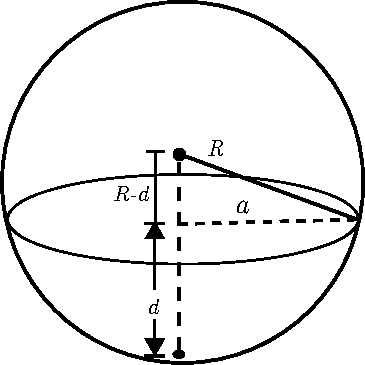
\includegraphics[width=.5\linewidth]{Chapters/Figures/SphericalCap}
	\label{fig:sphericalcap}
	\end{minipage}
\end{SCfigure}
Now, solving for $ \Delta A $ and using the above relationship in the last step, we find:
\begin{align*}
\Delta A &= 2\pi Rd - \pi a^2 \\
&= \pi(a^2+d^2) - \pi a^2 \\
&= \pi d^2
\end{align*}
 Rewriting (\ref{generic_surface_energy}), we can simplify surface energy in this geometry as 
 
 \begin{equation}
 \label{surface_energy}
 U_{surface} = \pi \Upsilon_{sv} d^2
 \end{equation}

\subsubsection{Force Balance}
At static equilibrium, the sum of the energies is:
\[U_{total} = \Upsilon_{sv} \pi d^2 + \frac{cER^{1/2}d^{5/2}}{1-\nu^2} - 2\pi W R d\] 
where c is a geometric factor to be determined in the next step. We can re-arrange the equation such that the sum of forces is equal to zero and differentiate both sides with respect to depth.

\begin{equation*}
\frac{\partial U_{total}}{\partial d} = \Sigma F = 0
\end{equation*}
\begin{equation}
\label{THEeqn}
2 \pi \Upsilon_{sv}d  + \frac{5cER^{1/2}d^{3/2}}{2 \left( 1-\nu ^2 \right) }  - 2 \pi WR = 0
\end{equation}
Here,  $ c = \frac{8}{5\sqrt{3}} $. This value of c is chosen to recover classical JKR theory, which predicts an indentation of $ d =  \left[\frac{\sqrt{3}\pi W (1 - \mu^2)}{2E} \right]^{2/3}R^{1/3}$ \cite{style2013surface, jensen2015wetting,johnson1971surface}. This energy balance was first published in 2013 by Style et al. in \textit{Nature Communications} \cite{style2013surface}. 

\subsection{Experimental Approach}
Equation \ref{THEeqn} gives us a quantitative relationship between the spontaneous indentation depth, $ d $, sphere radius, $ R $, and key material properties: $ \Upsilon, E, \nu, \text{and }W $. The Young Modulus, E, and the Poisson ratio, $\nu$ of the substrate can be measured separately for the substrate material. The depth $d$, and the radius $R$ of the sphere can be measured using fluorescent confocal microscopy, as described in section \ref{ch:microscopy}. The only remaining terms, $W$ and $\Upsilon$, the adhesion energy and the surface stress, respectively, can be determined with a two-parameter fit of $ d $ vs. $ R. $

\section{Preparing a Substrate}
In the following section, we outline the process of preparing a soft substrate for testing. The process is similar for a zero strain sample and a stretchable sample, and we make clear any distinctions between the two processes. Specific details for each substrate material tested can be found in Chapter 4.

Before preparing the substrate, we prepare the base surface on which the substrate will be coated. For a non-stretched sample, we use a glass coverslip, and for a stretched sample we use a thin, commercially available PDMS sheet from Specialty Manufacturing Incorporated. This base sheet is much stiffer ($ E\approx 1 $ MPa) than the substrate being tested.\todo[color=pink]{Check specs of sheet} We first coat this base layer with fluorescent beads in order to later locate the bottom of our substrate. In preparing our substrate, there are two important factors to consider: thickness and evenness of the surface. The substrate must be thick enough such that the the indenting spheres are not affected by the stiffness of the glass or PDMS base. This bottom layer of fluorescent beads allows us to easily gauge the thickness of our substrate. It is important that our substrate has an even surface, otherwise it is difficult to determine the sphere's depth, $ d $. To achieve this, we use a technique called spin-coating where we place our uncured substrate (when it still is a liquid) on the base and spin it rapidly for a period of time. The angular momentum  flings the fluid away from the center of the base. The result of this process is an even coating which will cure into our substrate over the next day.

Once cured, we deposit a second layer of fluorescent beads on the surface. These act as tracer particles which outline the indentation sphere. Using fluorescent confocal microscopy, we are able to precisely locate each fluorescent bead and outline the indentation sphere. It is important that the beads are dense enough to give a high resolution, yet not so dense as to become indistinguishable; this presents a challenge the MATLAB particle locating software. For a stretchable sample, we place the substrate, now cured onto the stretchable PDMS base, onto the lubricated stretching apparatus (described below). It is important remove any small bubbles on the stretcher's ring to ensure an airtight seal. 

The final preparation step is to sprinkle silica spheres of a range in size on top of the silicone. This should be done at least 30 minutes before collecting data so that the spheres have time to settle into an equilibrium state into the silicone. From a side view, the final setup should look like Figure \ref{fig:substrategraphic}.
\begin{figure}[h!]
	\centering
	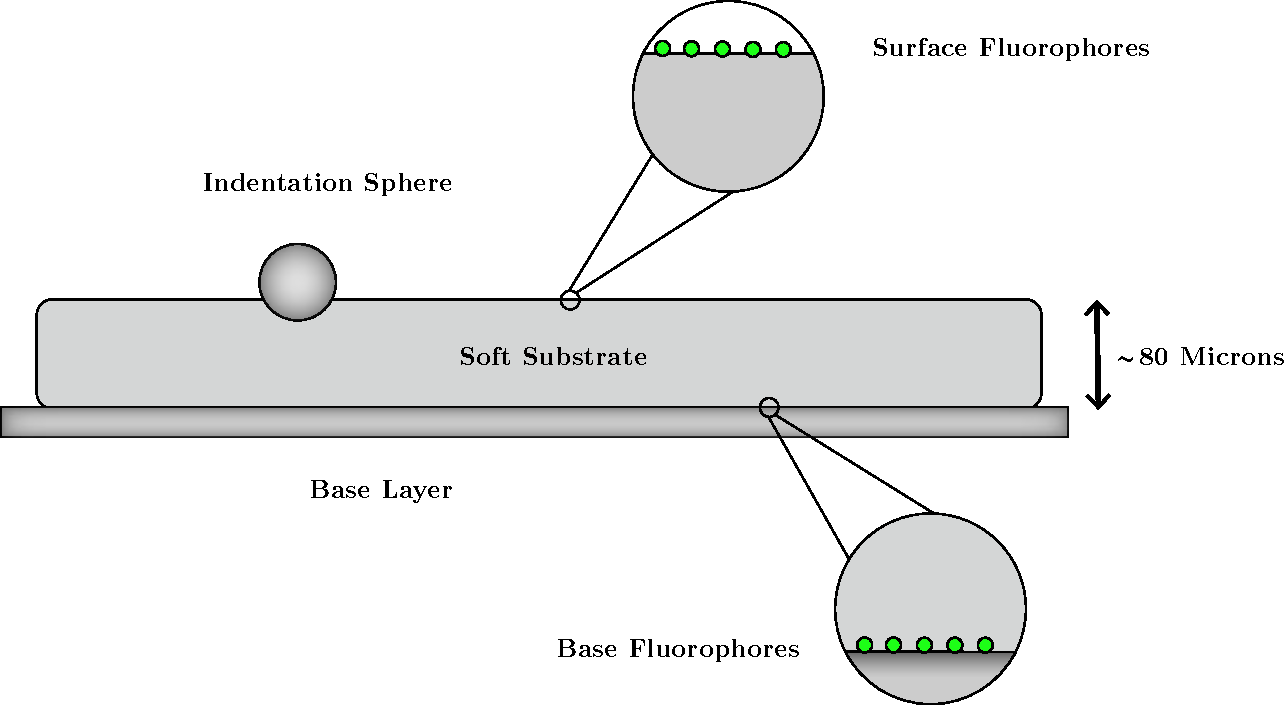
\includegraphics[width=.9\linewidth]{Chapters/Figures/substrate_graphic_new}
	\caption[Prepared Substrate Profile]{Above is the side profile of a prepared substrate sample. There are two layers of fluorescent beads: the bottom layer is used to measure the substrate's thickness, and the surface layer is used to outline the profile of the larger, indenting sphere. The soft substrate sits on an underlayer, namely glass or a stretchable PDMS silicone.}
	\label{fig:substrategraphic}
\end{figure}


\section{Stretching Apparatus}
Our interest is not just in  measuring $W$ and $\Upsilon$ for a given substrate, but in understanding how those values change when under strain. To accomplish this, we designed and built our own equibiaxial stretching apparatus capable of maintaining up to 35\% strain in our silicone samples. The design is based off of previous work designed for stretching biological tissues \cite{na2008time} and is similar in design to the apparatus used in the 2017 $\Upsilon(\epsilon)$ measurements \cite{xu2017direct}. Below is a general description of the design; detailed design documents can be found in Appendix A.

\subsection{Stretcher Design}
Geometrically, the stretching apparatus is constructed of two concentric cylinders connected at the base to create a channel between them. The top of each ring is flat, apart from a slight chamfer to reduce the risk of ripping the sheet as it is stretched. Each ring is then coated in Dow Corning vacuum grease to make a seal. It is critical that the inner ring has an ample amount of grease so that when a vacuum is pulled in the channel, the sheet will stretch from the center outwards  and not from the edges inwards. The sheet is held in place with an o-ring wrapped around the outside of the cylinder, which is then clamped down by a removable outer ring using a tension clamp. The tension provided by the o-ring and clamp ensure that a solid vacuum is kept and the edges of the sheet are minimally stretched into the trough.

\begin{figure}[h!]
	\centering
	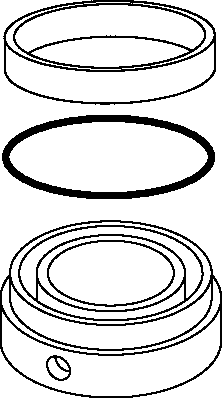
\includegraphics[width=.4\linewidth]{Chapters/Figures/exploded_stretcher}
	\caption[Stretching Apparatus Design]{Here is an exploded view of the stretching apparatus. The substrate goes on top of the base (substrate side down). It is then held down with an o-ring, which sits on the outside ledge. A second ring sits on top of the o-ring and is then held down by the microscope mount (not pictured here).}
	\label{fig:explodedstretcher}
\end{figure}
\begin{figure}[h!]
	\centering
	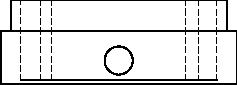
\includegraphics[width=0.6\linewidth]{Chapters/Figures/stretcher_side}
	\caption[Side Profile of Stretching Apparatus]{Above is the side profile of the stretching apparatus. Note the channel attached at the base, and the large center hole at the base where our substrate can be accessed by the microscope.}
	\label{fig:stretcherside}
\end{figure}


A tapped screw hole on the side of the apparatus connects the chamber to a syringe via thin, plastic tubing. To pull a vacuum in the channel, we withdraw air using a syringe pump. This allows us to have a consistent withdraw rate and control over the amount of air withdrawn to a high degree of precision. A deconstructive representation of the stretching apparatus can be found in Figure \ref{fig:explodedstretcher}.

\section{Calibration}
Originally, we intended to calibrate the strain value induced by the vacuum to the extent that we could predict the induced strain based on the amount of air withdrawn from the stretching apparatus. We withdrew air from the syringe and measured the movement of glass spheres adhered to the surface using a 10x air lens on our Nikon confocal microscope. Using the transmission detector allowed us to image the surface of our material with a wide field of view. Strain percentage was calculated using MATLAB code \cite{xu2017direct}.

There are several challenges in calibrating the induced strain. First, the stretching apparatus works best when a large strain is applied. Applying small strains one after another works but there is a threshold to induce stretch. No stretching change is visible if less than 2ml is withdrawn from the cylinder per increment. Thus, there is a limited resolution to our calibration data, which would not be a problem if the strain was linear. However, preliminary measurements indicated that the applied strain was nonlinear. This agrees with the with previous results \cite{na2008time} obtained using a similar device. Lastly, the greatest problem with calibrating strain is that we change substrates often. Even if we were to use the same exact sample, by removing it and setting up the device again, there is no way to standardize a zero-applied strain point. To prepare the stretching device, the sample is placed over the opening and a rubber o-ring is placed around the sample to help affix it in place. The sample must then be stretched and wiggled around slightly to remove any snags that could jeopardize the vacuum's efficacy. This means that every time a new sample is prepared, it is in an unknown and unique state of induced strain. Furthermore, before applying any strain, the substrate could be loose and uneven.

It was thus determined best to measure strain every time we applied a new strain to the silicone substrate and compare it to the substrate's original state. This also assured us that we knew the correct strain value to a higher precision for any given data set. Additionally, with the ability to hold strains exceeding 30\%, the 2mL resolution  limit became superfluous in seeking to measure $\Upsilon(\epsilon)$.


\subsection{Measuring Strain}
To determine the induced strain, we maximized the field of view. This allows us to see how more spheres are shifting, and thus gives a more accurate estimate of induced strain. As such, we decided to switch to the bright-field and measure how the spheres were shifting when stretched. We used a 10x air lens in conjunction with the transmission detector on our Nikon Confocal. We adjust the settings to give decent contrast, but it is more important to have the spheres in focus. For our Nikon this usually means setting the Power (HV) to 80. Each sphere reflects light, and it is this reflection that our particle locating software tracks after some image processing. An example image is located below (Fig.\ref{fig:TDpreandpost}), next to the same image after adjusting the contrast to help our tracking software with particle locating: 

\begin{figure}[h!]
	\begin{tabular}{cc}
		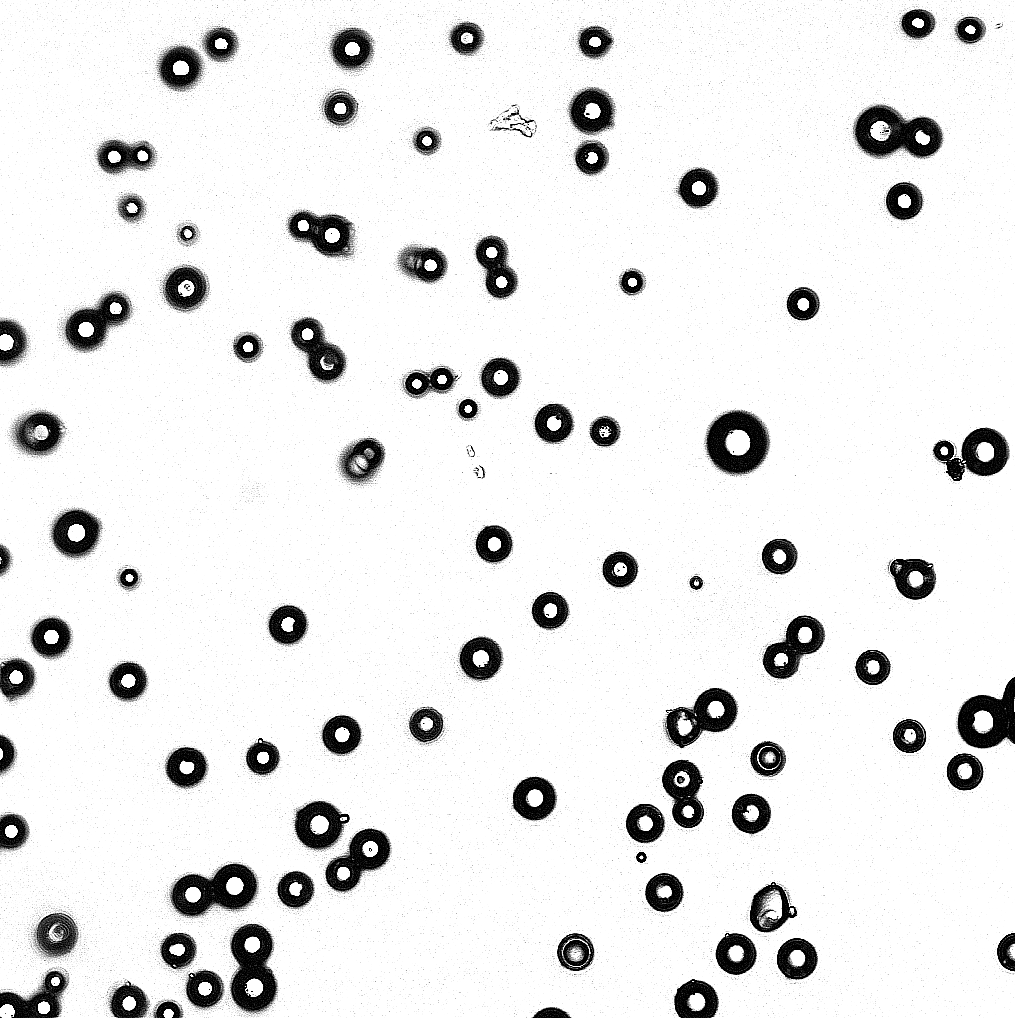
\includegraphics[width= .48\linewidth]{Chapters/Figures/181115_unstretched_b_thesis_contrast.png} & 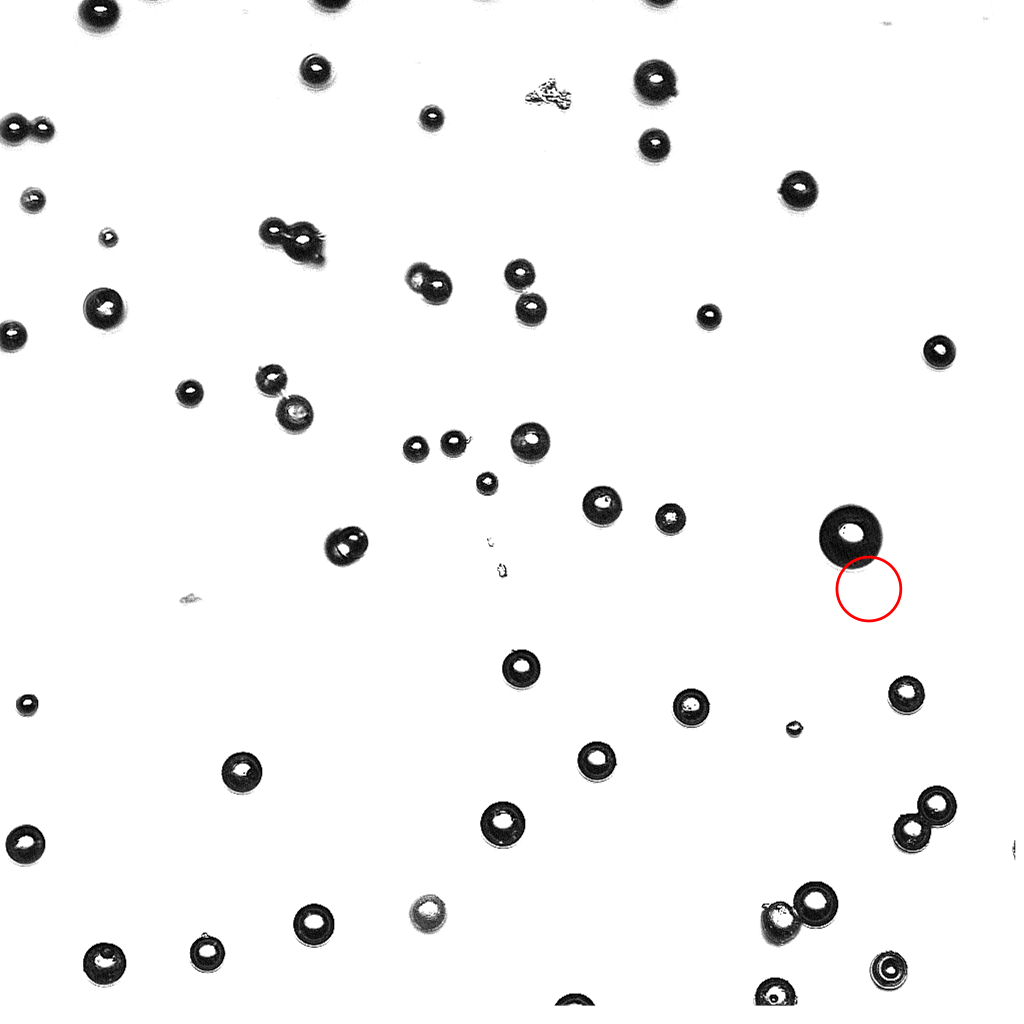
\includegraphics[width= .48\linewidth]{Chapters/Figures/181115_stretched_thesis_contrast.png}\\
		Fig. A & Fig. B
	\end{tabular}
	\caption[Bright-field pre and post image processing]{Add proper description}
		\label{fig:TDpreandpost}
\end{figure}

\begin{figure}[h!]
	\begin{tabular}{cc}
		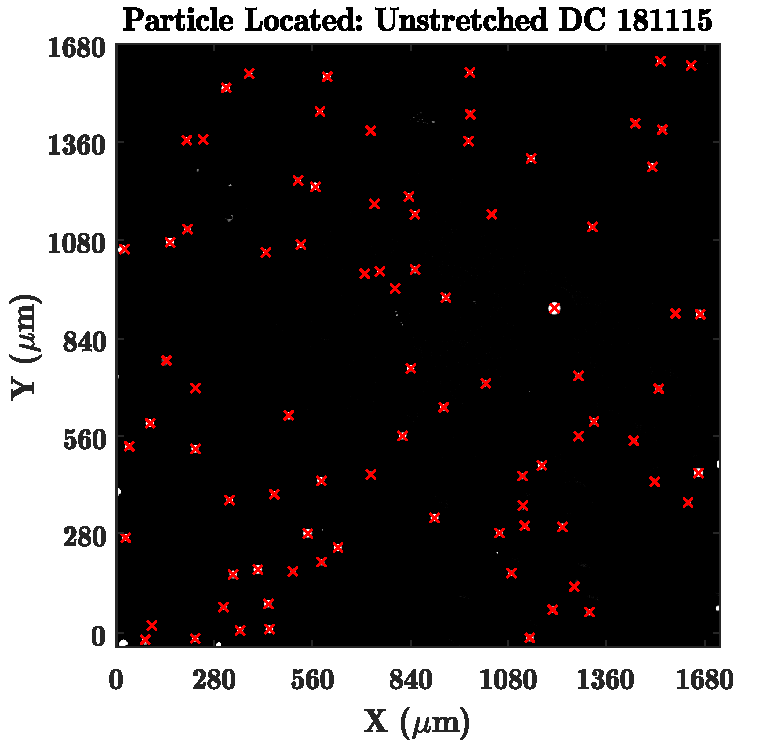
\includegraphics[width= .48\linewidth]{Chapters/Figures/particle_located_unstretched.pdf} & 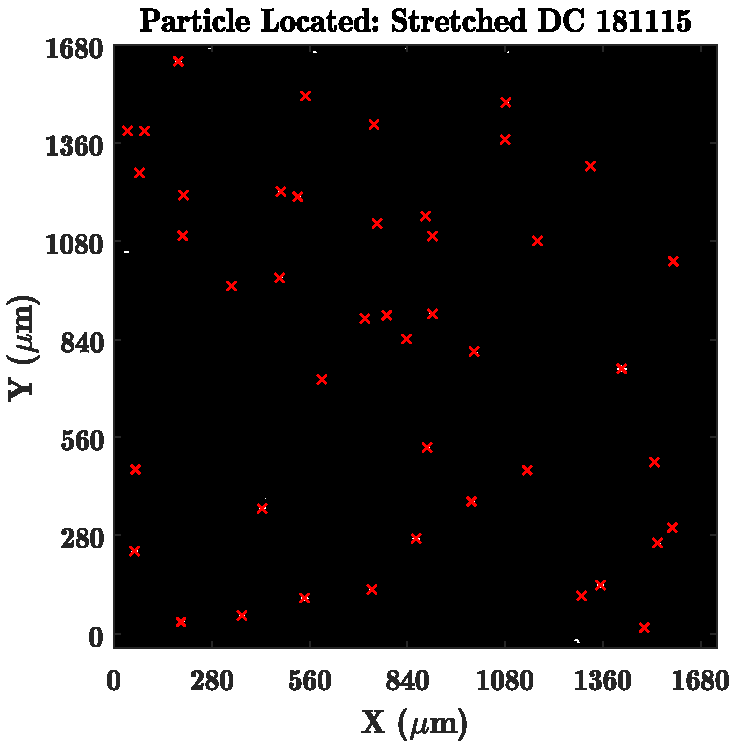
\includegraphics[width= .48\linewidth]{Chapters/Figures/particle_located_stretched.pdf}\\
		Fig. A & Fig. B
	\end{tabular}
	\caption[Bright-field pre and post image processing]{Add proper description}
	\label{fig:TDpreandpost}
\end{figure}


To track how the substrate stretches, we first find a centrally located group of spheres, or ``constellation.'' A good constellation is one that easily identifiable for relocation and tracking purposes, and one that has many discrete points in the field of view - i.e. there are plenty of non-overlapping spheres. It is an added bonus to find 4 spheres perpendicularly located, such that they form the tips of cross. Though not necessarily, this is useful for a preliminary strain calculation using the built in measuring functions on the Microscope's software. It is nice to track the progression of stretching and ensure the substrate is not preferentially stretching in on direction; this could indicate the substrate is caught in the apparatus. Not only does this ruin the symmetry assumptions being made for our calculation, but it could lead to the substrate tearing if more strain is being applied than expected.

To evacuate the cylinder, we use the the Harvard Apparatus\texttrademark \ Elite Pro Syringe Pump with a 50mL Luerlock syringe. Before beginning any stretching, we withdraw a few ml of air to ensure the substrate is flat and not sagging. At this point we take a picture of the brightfield and call it the ``zero applied strain'' image. We compare all stretched data to this image in order to determine the induced strain. Because of the geometry of the stretching apparatus, along with the way the silicone cures and the local strains induced by adhesion, we do not yet have a way to determine the true strain of the silicone. However, we are most interested in the slope of the $\Upsilon$ vs. $\epsilon$ curve, $\Lambda$, so this is not vitally important.

The induced strain is a tensor of rank two. Because we are stretching the substrate equally in all directions, we can just look at the magnitude of the tensor and treat the strain as a scalar \cite{xu2017direct,xu2018surface}.     


\begin{figure}[h!]
	\centering
	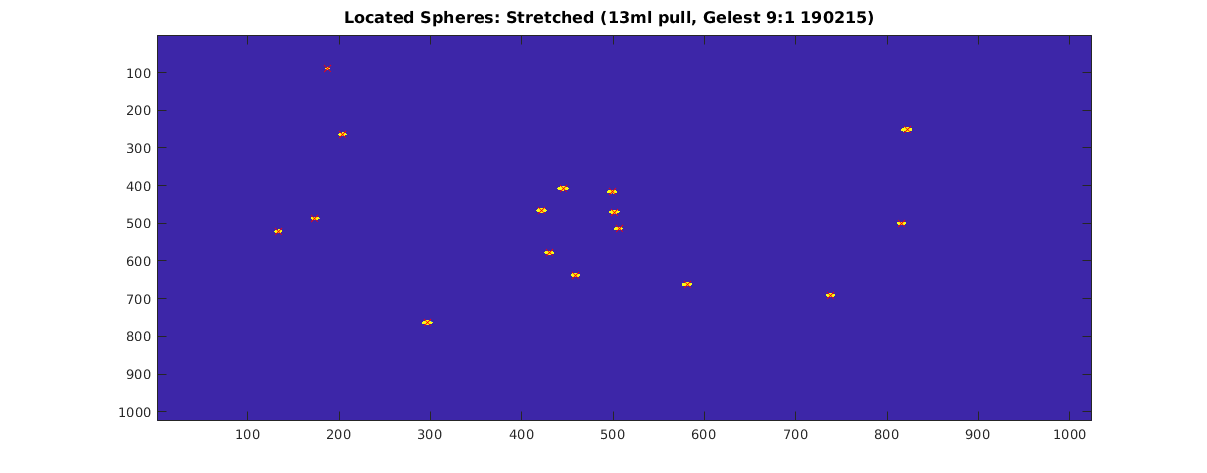
\includegraphics[width=\linewidth]{Chapters/Figures/13ml_stretched_2D_located}
	\caption[Unstretched]{}
	\label{fig:13mlstretched2dlocated}
\end{figure}

\begin{figure}[h!]
	\centering
	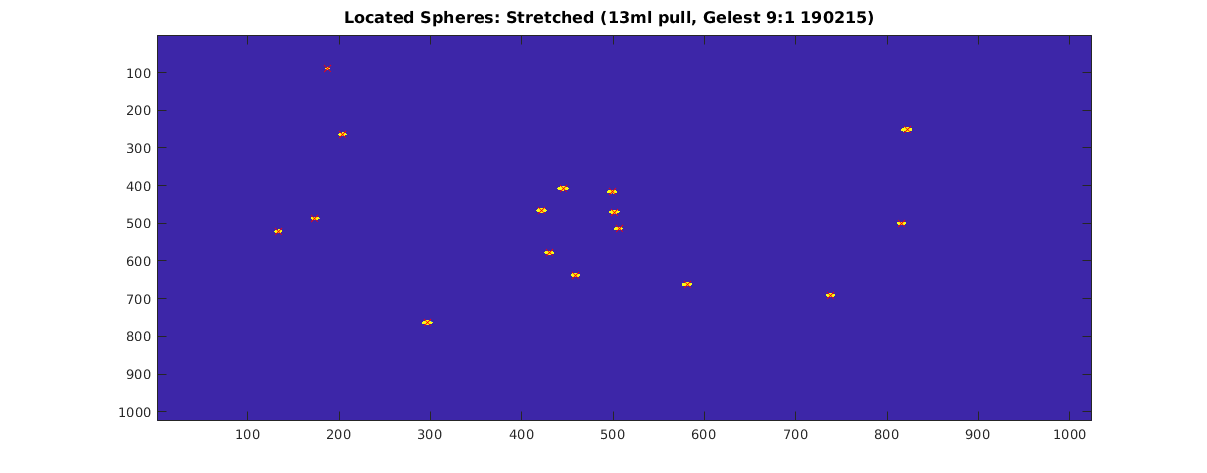
\includegraphics[width=\linewidth]{Chapters/Figures/13ml_stretched_2D_located}
	\caption[Stretched]{These are placeholders for now. I don't really like how they look and I don't think they're totally necessary. It might be nice to keep them if I can clean them up. Especially if I get some nice stretch data with the new DC}
	\label{fig:13mlstretched2dlocated}
\end{figure}
\todo[inline,color=pink]{There's an alternate image where each point is an x for before after. Replace figure with that and zoom in on sphere cluster.}

\section{Material Characterization}
To measure the stiffness of our substrate, we do not use the confocal measurement sample. Instead, when preparing the sample, we cure a surplus of the substrate material in a vial to test the bulk characteristics of the sample. 

We take a standard bulk stiffness measurement using the Texture Technologies TA.XT Plus texture analyzer. A rigid cylinder with radius $R = 1.5$ mm is slowly indented into the bulk substrate. The force response vs. indentation depth is recorded for several tests with varying starting heights and locations (See Figure \ref{fig:Bulkstiffness_raw}). We use the average E value obtained from these tests in our W,$ \Upsilon $ fitting. The fitting processed will be reviewed in Chapter 3. 


\subsection{Hertzian Contact Mechanics Derivation}
We calculate the Young's modulus for the bulk sample using classic Hertzian contact mechanics between a flat, rigid cylinder and an elastic half-space.

\begin{equation}
F=2RE^*d
\end{equation}
where 
\begin{equation*}
\frac{1}{E^*} = \frac{1-\nu_1^2}{E1} + \frac{1-\nu_2^2}{E2}
\end{equation*}
Here, we are working with a large indenter and a geometry that fixes the contact area. For Silicone, $ \nu \approx .5$ for low strains; for the rigid cylinder, $ E \gg 1-\nu^2 $, so we can ignore that term. From the Force vs. depth information, we can write an equation for E:

\begin{align}
&\frac{1}{E^*} = \frac{2Rd}{F} \\
&\frac{1 -\nu^2}{E} = \frac{2Rd}{F} \\
&E = \frac{\left( 1-\nu^2 \right) F}{2Rd} \\
&E = \frac{\left( 1-.5^2 \right) F}{2(1.5 \cross 10^{-3})d}
\end{align}
\todo[color=pink]{Equation alignment doesn't look right}

\begin{figure}[h!]
	\centering
	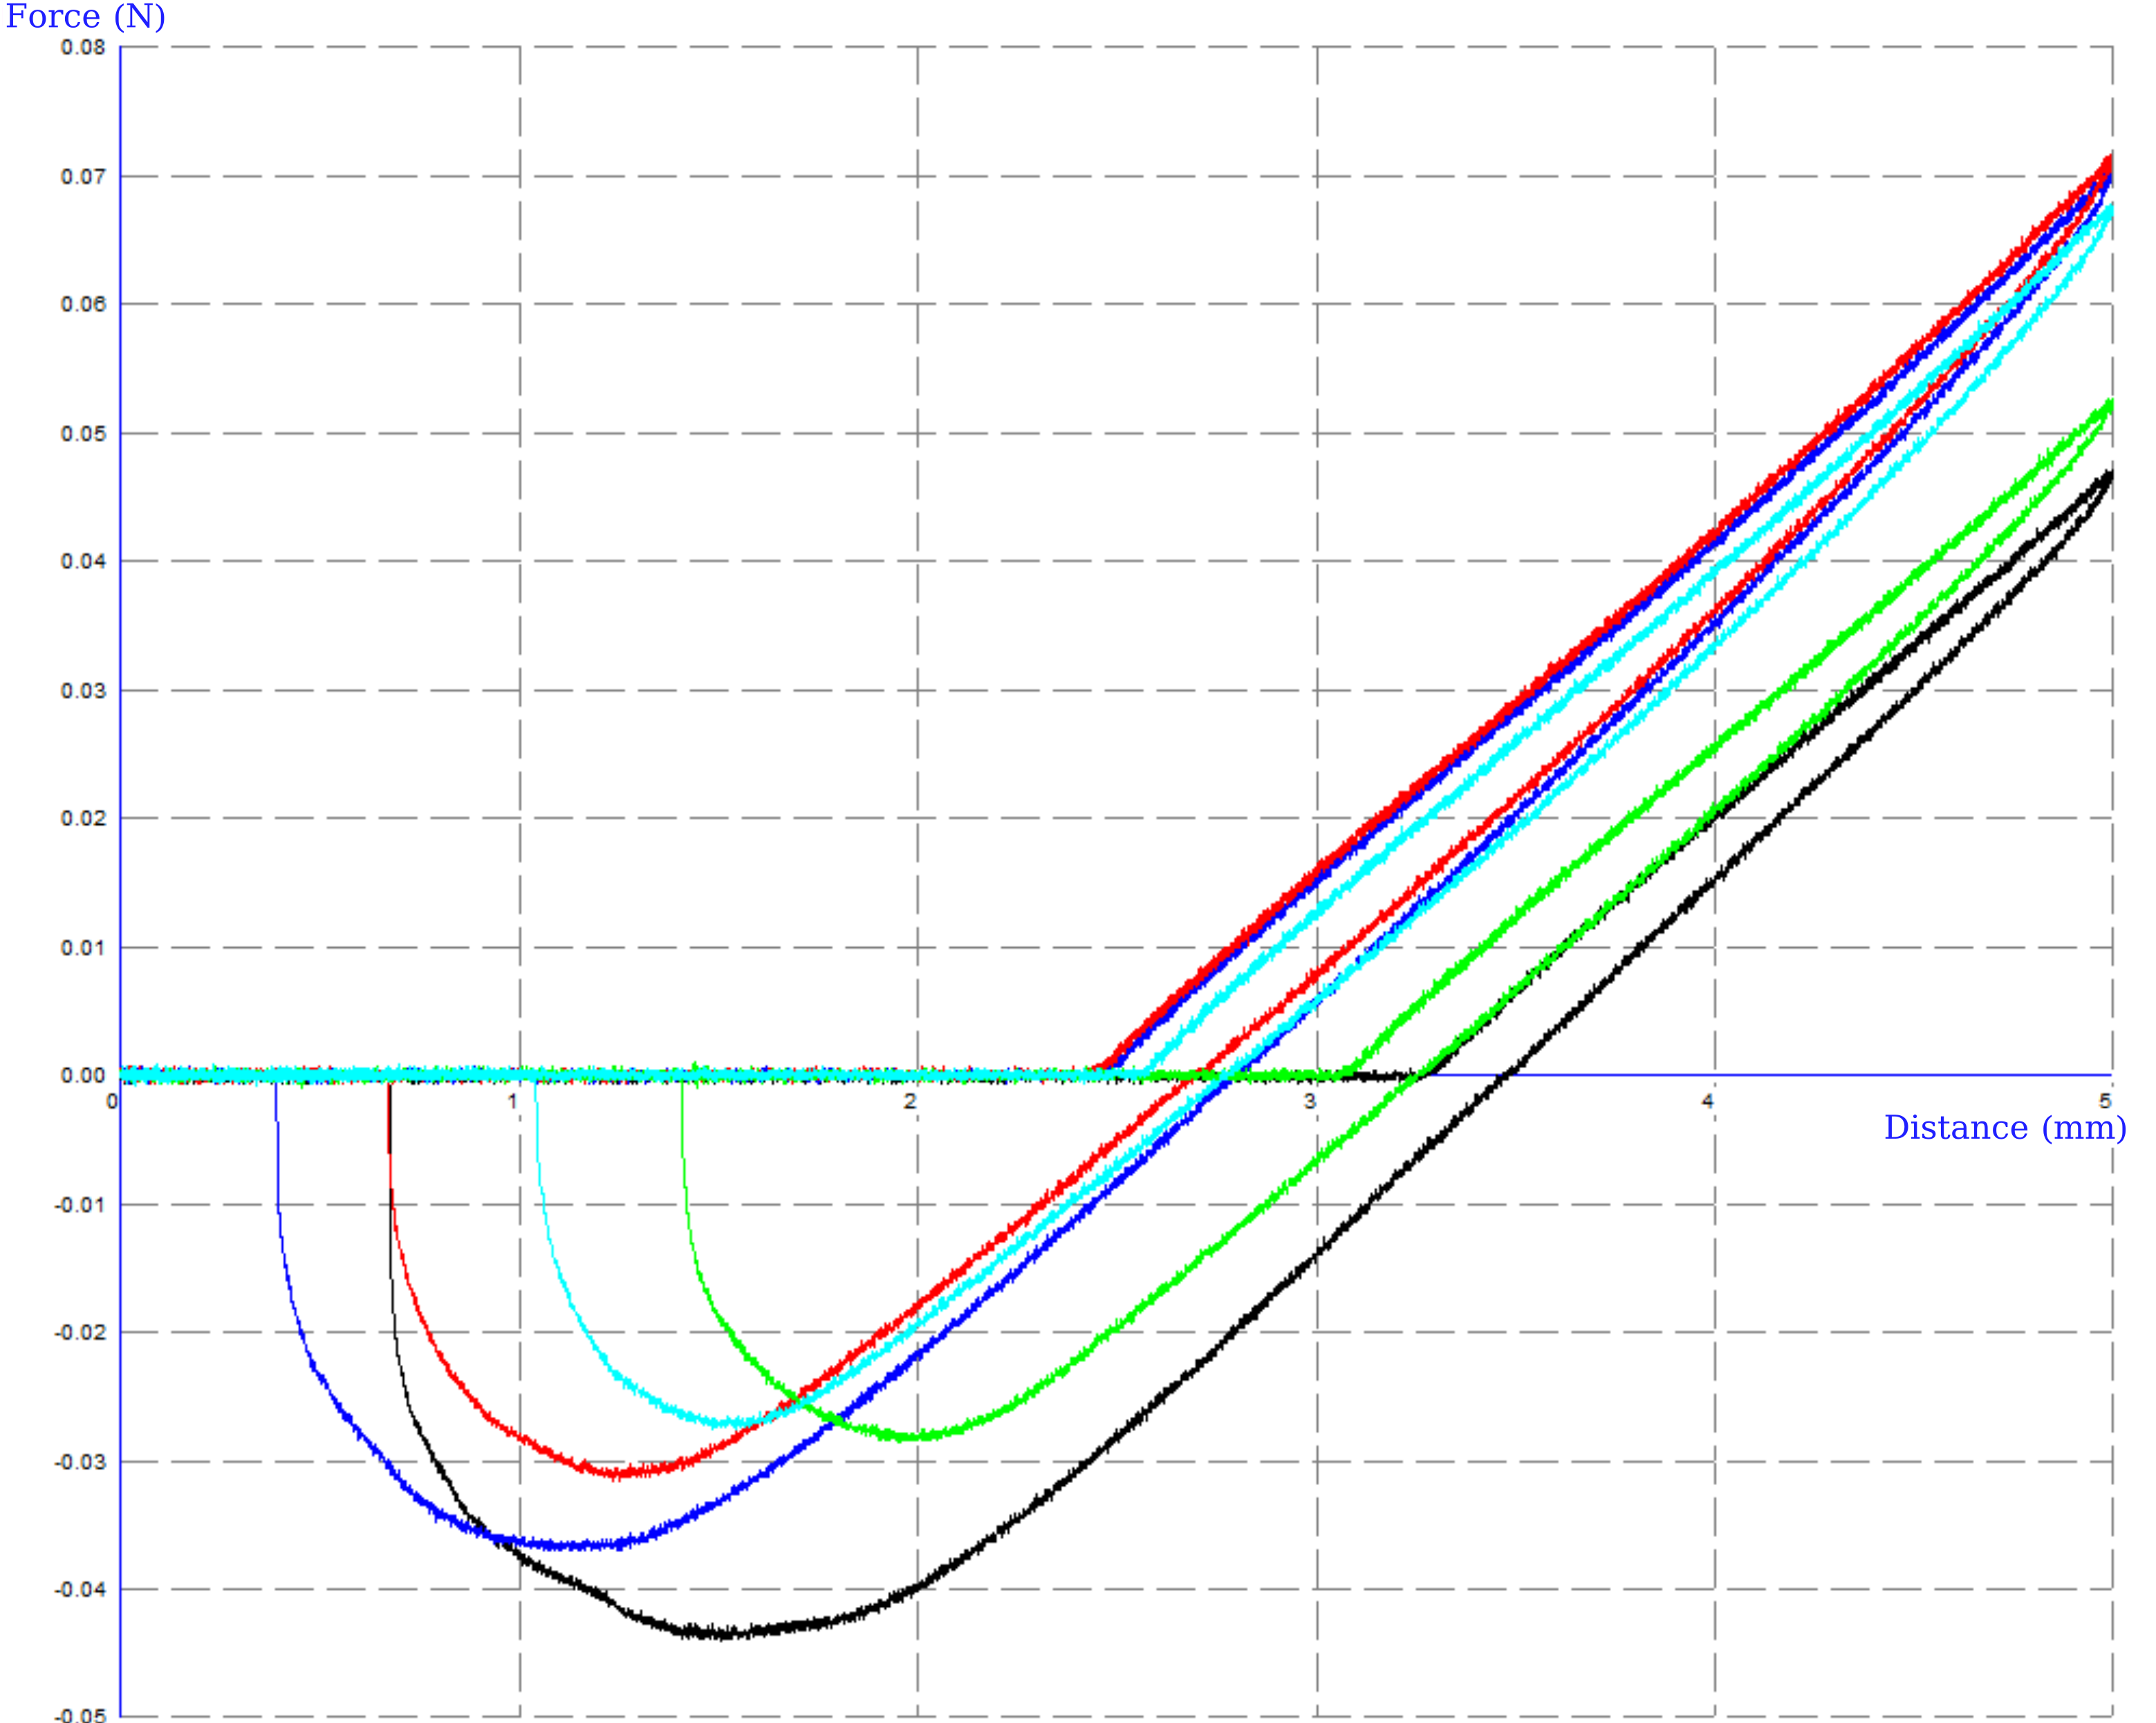
\includegraphics[width=\linewidth]{Chapters/Figures/190406_DC_1-1RT1-5.png}
	\caption[Bulk Modulus Test]{Force vs indentation depth for a bulk sample of silicone. Each color represents a separate measurement at varying starting heights and locations on the sample.\todo[inline, color=pink]{Do you think the axis values are too small? I haven't seen this printed yet.}}
	\label{fig:Bulkstiffness_raw}
\end{figure}

\section{Putting it all Together}
Using the texture analyzer, we can measure $ E $ for our substrate. Next, we need a way to measure $ d $ vs. $ R $ for many spheres per sample. With these three values measured, only two terms in Equation \ref{THEeqn} remain unknown, $ \Upsilon $ and $ W $. To determine these unknown values, we can run a two parameter fit using Equation \ref{THEeqn}. Using our equibiaxial stretching apparatus, we can then repeat the $ d $ vs. $ R $ measurements at a range of strain to determine $ \Upsilon(\epsilon) $. The process of collecting the $ d $ vs. $ R $ measurements for a single sphere is explained in Chapter 3.

%